\chapter{Validation}
During the model validation process the model's performance and consistency is tested. This helps to detect any potential weaknesses or shortcomings in the model and provides an opportunity for improvement.

Important components of model validation are:

\begin{itemize}
  \item Data Quality Assessment: Evaluating the quality, completeness, and reliability of the data used to build the PD model, including their data sources.  
  \item Model Performance Evaluation: Assessing the model's predictive power and discrimination ability, which is usually analysed by the following metrics: Area Under the Receiver Operating Characteristic curve (AUC-ROC), accuracy, precision, recall, and F1-score. 
  \item Sensitivity Analysis: Analysing the impact on the result of the model for different changes in the input variables. This helps identifying the most influential factors and potential vulnerabilities of the model.
  \item Robustness Testing: Examining the model's stability and performance under different scenarios and stress conditions. This involves stress testing the model with extreme cases or outlier data points to assess its resilience and reliability.
\end{itemize}

\section{Out-of-Sample and Out-of-Time Validation}
Out-of-sample validation involves testing the model's performance on a data set that was not used during model development. Out-of-time validation goes one step further, it includes new data which covers additionally a different, more current time period. An illustration is depicted in Fig. \ref{fig:vl_valsample}. The purpose is to assess the model's ability to make accurate predictions on new, unseen data. Because the model is estimated on the training sample, it is common that the model shows a better performance on in-sample data sets than on another sample. However, if the performance metrics differs significantly, this could be seen as a sign of over-fitting. 

\begin{figure}[H]
	\centering
	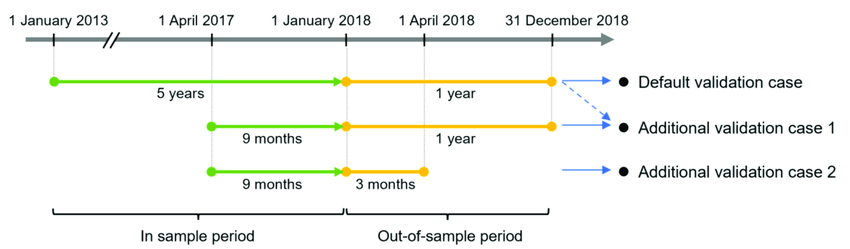
\includegraphics[width=0.625\textwidth]{./VL__validationsample.png}
    \caption{Selection of out-of-sample and out-of-time sample}
    \label{fig:vl_valsample}
\end{figure}

The full data set is usually split into 70\% training and 30\% testing sample, also called validation sample. Different ratios, e.g. 60/40, 80/20, are also popular and mainly depends on the size of the data set and number of default events. During the splitting process it is important to keep the number of default events even in both samples to prevent situations, where one class is disproportionate to the other. This process is called stratification, visible in Fig. \ref{fig:vl_strat}. It ensures that there will be no biased model training and evaluation. 

\section{Model Performance Evaluation}
Popular metrics to assess the discriminatory power of rating systems are Confusion Matrix, Area Under the Receiver Operating Characteristic Curve (AUC-ROC Curve), Gini coefficient, Cumulative Accuracy Profile (CAP) and its summary index, the Accuracy Ratio (AR). 

\subsection{Confusion matrix}
The confusion matrix is a table with four elements (Fig. \ref{fig:vl_confmatr}), it shows the number of observations which have been correctly (True Positive, True Negative) and incorrectly (False Positive, False Negative) identified as default or non-default.A False Positive, meaning a customer was predicted to default but survived, is also called Type I Error and aFalse Negative, thus a borrower is expected to survive but defaulted, is also known as Type II error. In practice, a Type II error is more severe, because the loss caused by a defaulted exposure is higher than the lost opportunity income due to a rejected non-defaulted application. For the transformation from PD to a default flag a cut-off has to be selected. To determine an ideal cut-off, the F1-Score can be utilized, where the cut-off value is set where the F1-score is maximised.

\begin{figure}[H]
	\centering
	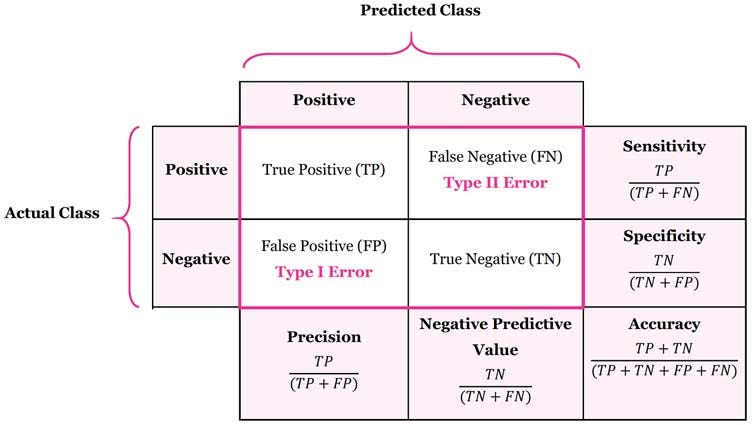
\includegraphics[width=0.625\textwidth]{./VL__confmatrix.jpg}
    \caption{Confusionmatrix}
    \label{fig:vl_confmatr}
\end{figure}

Using the elements of the confusion matrix, the measures Accuracy, Precision, Recall, F1-Score and others can be calculated, visible in Eq. \ref{eq:vl_sens} to \ref{eq:vl_f1}. However, measures like Accuracy and Precision are not recommended for unbalanced data because they can provide misleading insights about model performance. In the case of unbalanced data, where one class is significantly larger, a model can achieve high accuracy by simply predicting only the majority class. This high accuracy overshadows the model's ability to correctly identify observations of the minority class. Recall and F1-score provide a more accurate view.

\begin{flalign} 
\text{Sensitivity} &= \frac{\text{True Positives}}{\text{True Positives} + \text{False Negative}} \\[10pt] \label{eq:vl_sens}
\text{Specificity} &= \frac{\text{True Negative}}{\text{True Negative} + \text{False Positives}} \\[10pt]
\text{Precision} &= \frac{\text{True Positives}}{\text{True Positives} + \text{False Positives}} \\[10pt]
\text{Negative Predictive Value} &= \frac{\text{True Negative}}{\text{True Negative} + \text{False Negative}} \\[10pt]
\text{Accuracy} &= \frac{\text{True Positives} + \text{True Negatives}}{\text{Total Population}} \\[10pt]
\text{Recall} &= \frac{\text{True Positives}}{\text{True Positives} + \text{False Negatives}} \\[10pt]
\text{F1-Score} &= 2 \times \frac{\text{Precision} \times \text{Recall}}{\text{Precision} + \text{Recall}} \label{eq:vl_f1}
\end{flalign}

\subsection{Receiver Operating Characteristic Curve}

The Receiver Operating Characteristic Curve (ROC Curve) is the resulting curve after plotting the proportion of False Positive along the x-axis and proportion of True Positive along the y-axis. A diagonal line between (0,0) and (0,1) represents the random model and the curve of a perfect model would be a step function that goes from (0,0) straight up and moves horizontally to (1,1). The Area Under the ROC-Curve (AUC-ROC Curve) is, as the name suggests, the area below the ROC-curve. The areas are marked as A and B in Fig. \ref{fig:vl_roccurve} and the formula is seen in Eq. \ref{eq:vl_auc}.

\begin{equation}
AUC = A + \frac{1}{2} \label{eq:vl_auc}
\end{equation}

\begin{figure}[H]
	\centering
	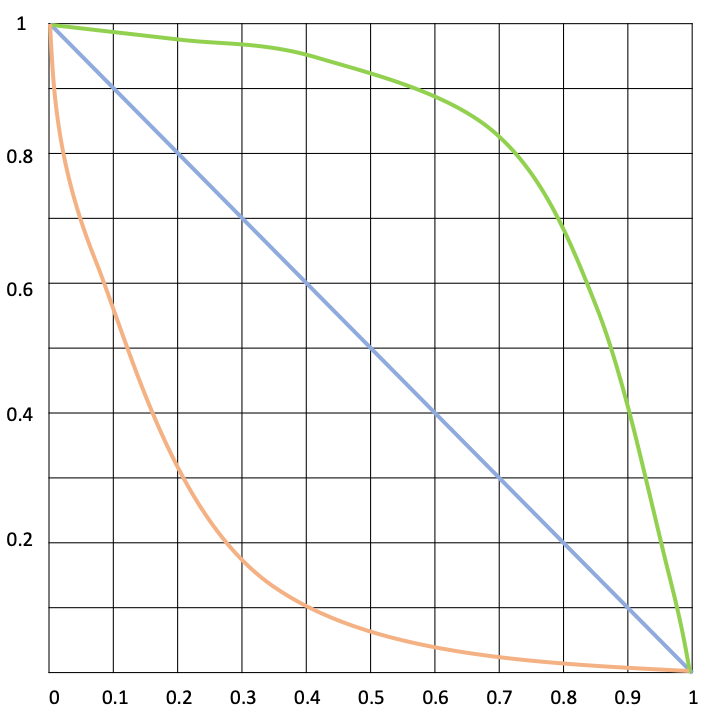
\includegraphics[width=0.625\textwidth]{./VL__ROC_curve.png}
    \caption{ROC curve}
    \label{fig:vl_roccurve}
\end{figure}

\subsection{GINI coefficient}
\label{sec:gini}
The Gini coefficient and AUC are connected via the formula Eq. \ref{fig:vl_gini} and a visual presentation is visible in Fig. \ref{fig:vl_gini}. Therefore, they relate the same information but are differently scaled. The Gini coefficient shows an improved interpretability. While the AUC has a range between 0.5 (random model) to 1 (perfect model), the Gini coefficient takes on values between 0 (no discriminatory power) and 1 (perfect discriminatory power). Generally, the AUC can also take on a value below 0.5, but that would indicate, that the model's predictions is worse than the random model and therefore imply an issue in the model's ability to differentiate between the classes. 

\begin{equation}
GINI = \frac{A}{A + B} = \frac{A}{\frac{1}{2}} = (2 * A + 1) - 1 = 2 * \text{AUC} - 1 \label{eq:vl_gini}
\end{equation}

\begin{figure}[H]
	\centering
	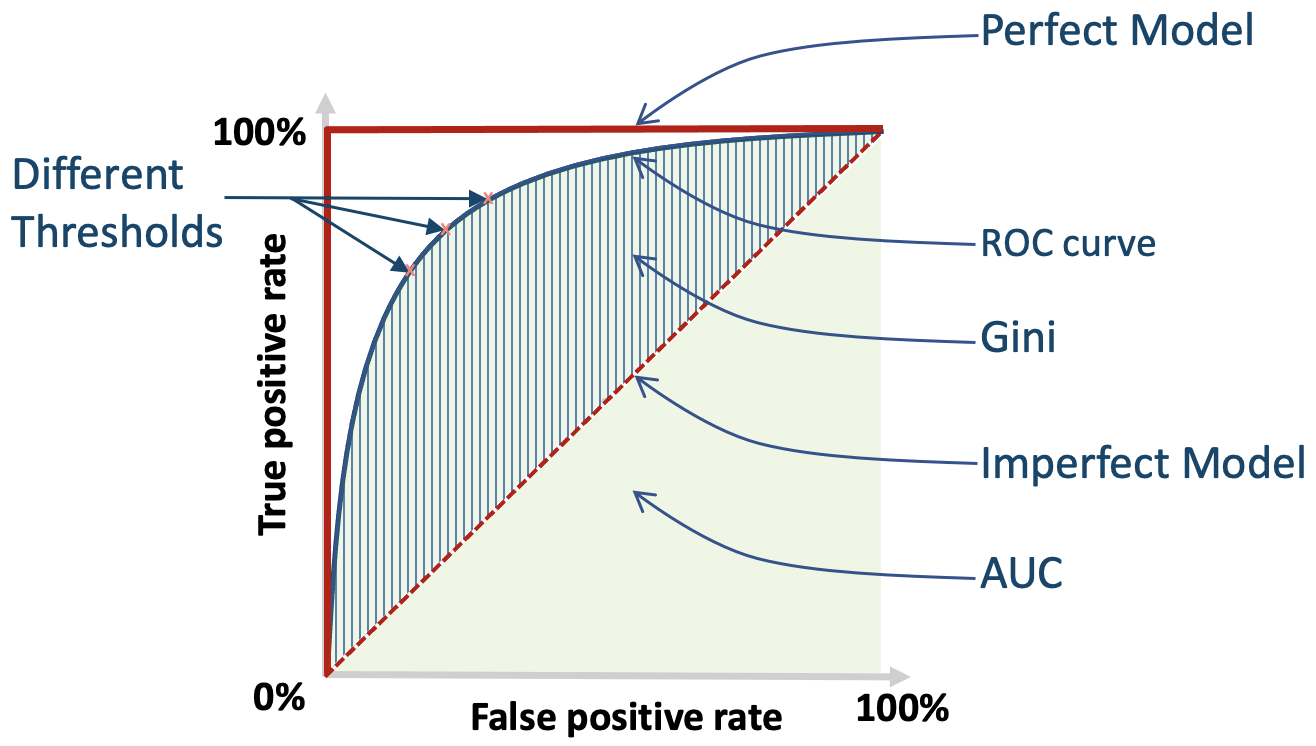
\includegraphics[width=0.625\textwidth]{./VL__gini.png}
    \caption{GINI coefficient}
    \label{fig:vl_gini}
\end{figure}

\subsection{Cumulative Accuracy Profile}

In the CAP-graph the percentage of all borrowers are plotted along the x-axis and the percentage of defaulted borrowers are plotted along the y-axis (Fig. \ref{fig:vl_cap}). The resulting curve is a way to assess how well the model differentiates between the two groups, comparing the performance to the perfect or random model. The Accuracy Ratio is the ratio of the area between the analysed and random model divided by the area between perfect and analysed model (Eq. \ref{eq:vl_ar}). 

\begin{equation}
Accuracy Ratio = \frac{A}{A + B} \label{eq:vl_ar}
\end{equation}

\begin{figure}[H]
	\centering
	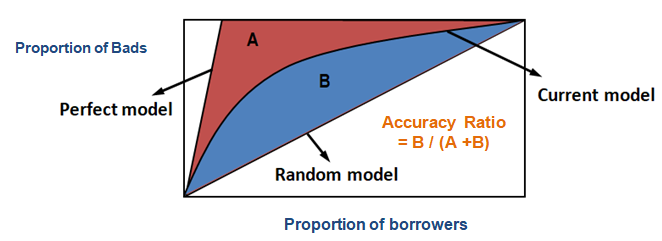
\includegraphics[width=0.625\textwidth]{./VL__CAP.png}
    \caption{Cumulative Accuracy Profile}
    \label{fig:vl_cap}
\end{figure}

\section{Stability Test}
Stability testing is performed to assess the robustness and consistency of a PD model over time. It examines whether the model's performance remains stable and reliable when applied to data collected at different time periods. Stability testing helps to identify potential model deterioration or drift over time, which may be caused by changes in the underlying credit conditions or data characteristics. If significant discrepancies are detected, model recalibration or updates may be necessary to maintain its accuracy and relevance.